\subsection{Alloy}
% Set Language
We have used the functionalities provided by the Alloy tool in order to represent the domain assumptions of our System. 
The model, as we will see, represents a snapshot of the System at a given time.
All the interesting part of the code are commented in order to better explain their meaning.

We have also added some interesting predicates to show some possible world which is not in contrast with our assumptions.

\subsubsection{Gps Utilities}
\alloyfile{../Alloy/Exported/GeoUtilities.als}
In this file, we have modelled the GPS positions that our System has to cope with.

Given our domain assumptions, positions are exact for CompanyArea because they are predefined. In the reality, it does mean that each Parking Area or Charging Area has a given and exact set of GPS points denoting the volume it occupies.

On the other hand, GPS positions for Persons and Cars are derived from devices and they are not always accurate.
For this reason, we introduced the concept of GpsVolume, consisting of various GpsPoints, and that should be read as "the volume that a Person/Car can occupy at a given moment basing on their GPS coordinates". It basically means that, knowing the GPS coordinates of a person at a given moment, we built a probabilistic assumption of the volume in space he/she is occupying. Obviously the same concept applies for the cars. 

For the reasons explained above, in our model we have can have different Persons and/or Cars in the same GpsVolume. 

To model the fact that persons or cars are nearby we say that they have to share at least one GpsPoint. So if a Person is inside a Car he/she should have some GpsPoint in common with it; the same concept applies for Cars inside CompanyAreas.

We will clarify these aspects in the following pages.

As a last note, we assume that two different GpsVolumes have at least one different GpsPoint.

A simple world is shown in Figure \ref{fig:GpsWorld}

\begin{figure}[!htbp]
\centering
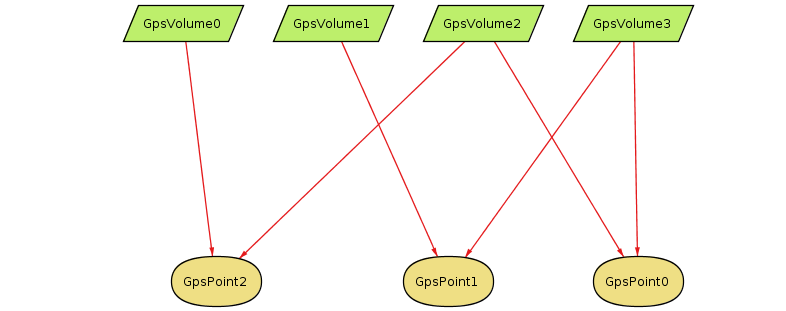
\includegraphics[max size={\textwidth}{\textheight}, keepaspectratio]{../Alloy/Exported/Images/GpsWorld.png}
\caption{A Gps World}
\label{fig:GpsWorld}
\end{figure}
\FloatBarrier

\subsubsection{Persons}
\alloyfile{../Alloy/Exported/Persons.als}

In this file, we have modelled the different kind of people that our System should cope with. In our model, we are not interested in Visitor, so we model simply Persons (general people) and Users (Persons registered to our System).

Figure \ref{fig:PersonsWorld} shows a possible world generated by our Alloy code. We note, for example, that \textit{User0} and
\textit{Person1} are both linked to \textit{GpsVolume3}: as we have said before, this is not in contrast with our model.

\begin{figure}[!htbp]
\centering
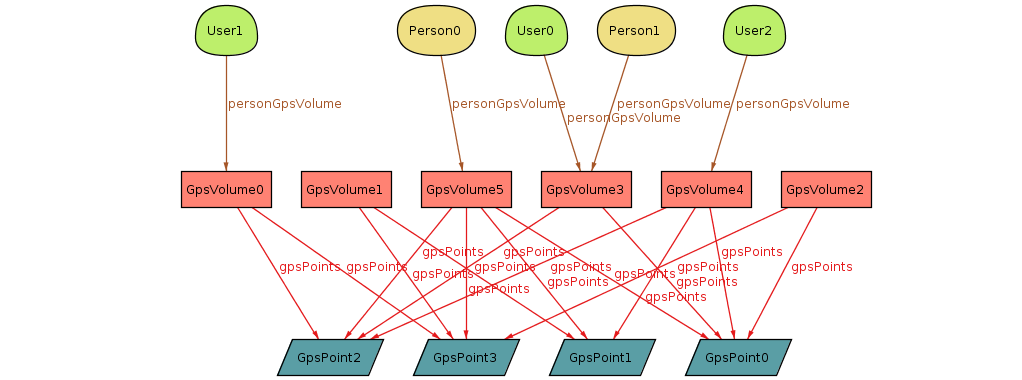
\includegraphics[max size={\textwidth}{\textheight},keepaspectratio]{../Alloy/Exported/Images/PersonsWorld.png}
\caption{A Persons World}
\label{fig:PersonsWorld}
\end{figure}

The \textit{showCouldExistNearbyPersons()} predicate is used to show what we have defined as nearby people: two Persons sharing at least one GpsPoint. This is shown in figure \ref{fig:PersonsNearby}, where we can see that \textit{User1} and \textit{User2} are nearby.

\begin{figure}[!htbp]
\centering
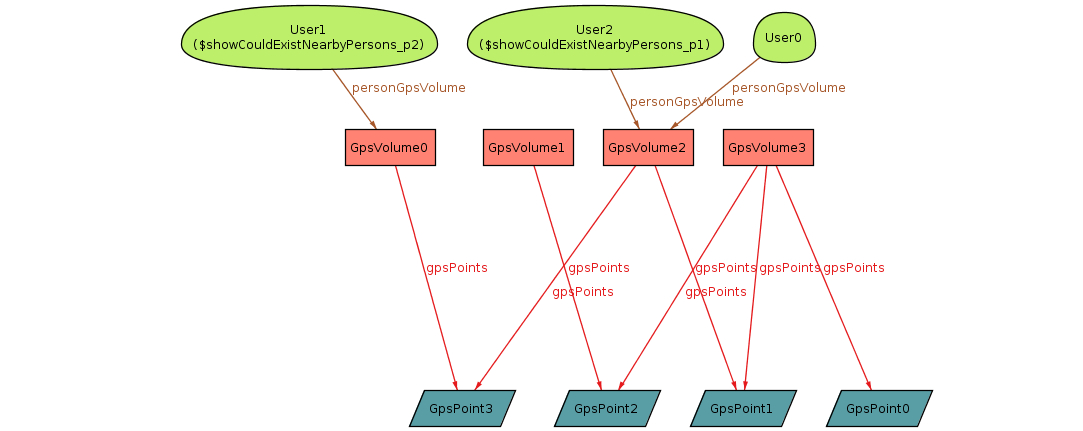
\includegraphics[max size={\textwidth}{\textheight},keepaspectratio]{../Alloy/Exported/Images/PersonsNearby.png}
\caption{Nearby Persons}
\label{fig:PersonsNearby}
\end{figure}
\FloatBarrier

\subsubsection{Cars}
\alloyfile{../Alloy/Exported/Cars.als}

In this piece of code we show our model for the Cars managed by our System; a possible world is shown in figure \ref{fig:CarsWorld}. We can note that there is a single car, characterized by
\begin{itemize}
	\item a PluggedOff status: this is consistent since the car is also InUse;
	\item an EngingOn status: as for the above, this is consistent since the car is also InUse;
	\item two different MinorDamages: this is consistent since Users can also use Cars that have minor damages;
	\item a LowBattery: this is consistent since the car is InUse; when the Car will be parked, its status, according to our assumptions, will be set to Unavailable
	\item two CarSeats: they are occupied by an User and a Person, that are both nearby our Car (i.e. they have at least one GpsPoint in common with our Car).
\end{itemize}

\begin{figure}[!htbp]
\centering
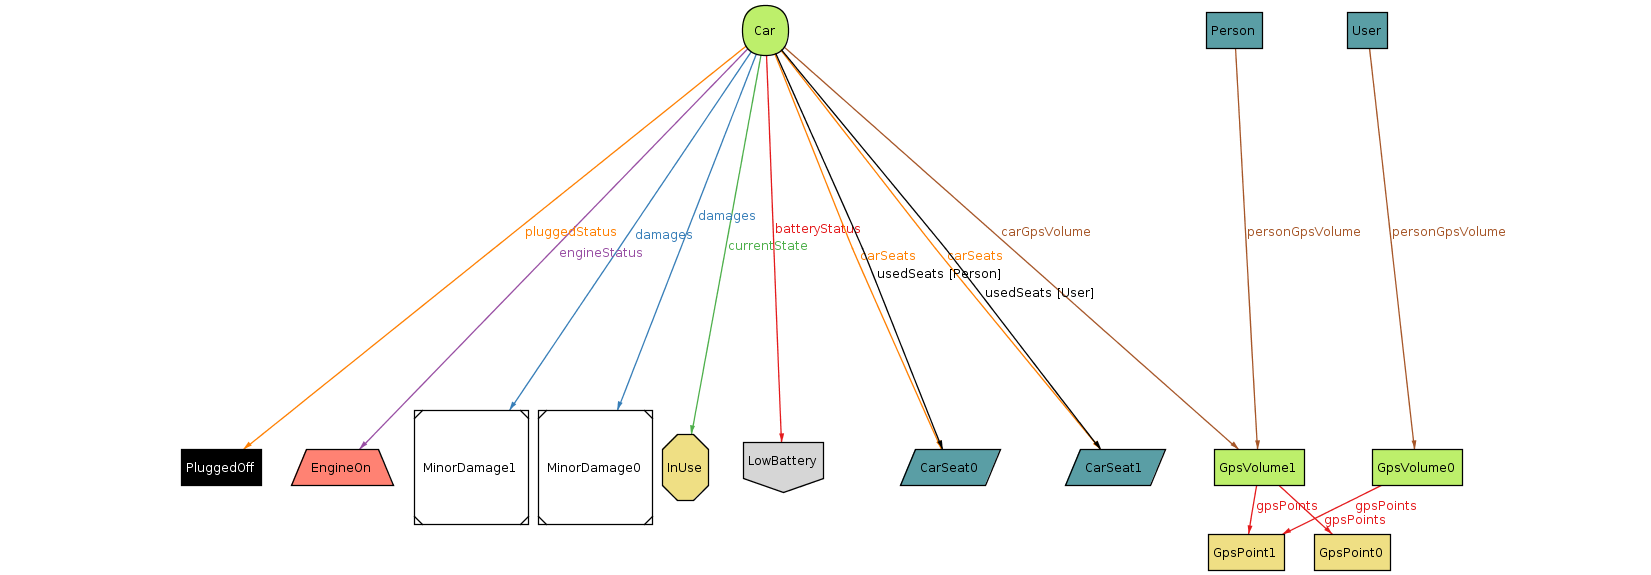
\includegraphics[max size={\textwidth}{\textheight},keepaspectratio]{../Alloy/Exported/Images/CarsWorld.png}
\caption{A Cars World}
\label{fig:CarsWorld}
\end{figure}

We have also shown in \ref{fig:CarsExecution} that the execution of all the assertions have not generated counterexamples, so we can assume reasonably assume that our model is consistent.
\begin{figure}[!htbp]
\centering
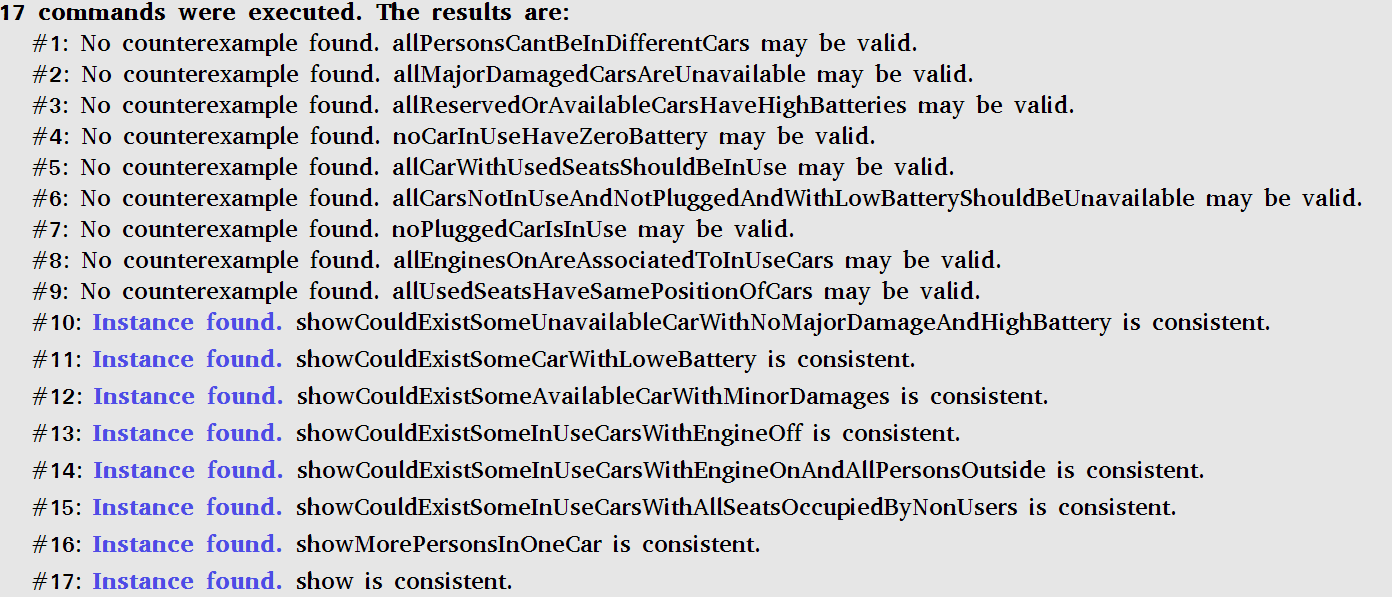
\includegraphics[max size={\textwidth}{\textheight},keepaspectratio]{../Alloy/Exported/Images/CarsExecutions.png}
\caption{Executions of checks and predicates for Cars}
\label{fig:CarsExecution}
\end{figure}

An important aspect of our System is that a Car can be In Use, but with no person inside it. The world for this scenario is represented in Figure \ref{fig:CarsNoneInside}. Another interesting aspect shown in this image is that, although no one is inside the Car, its engine is still on.

\begin{figure}[!htbp]
\centering
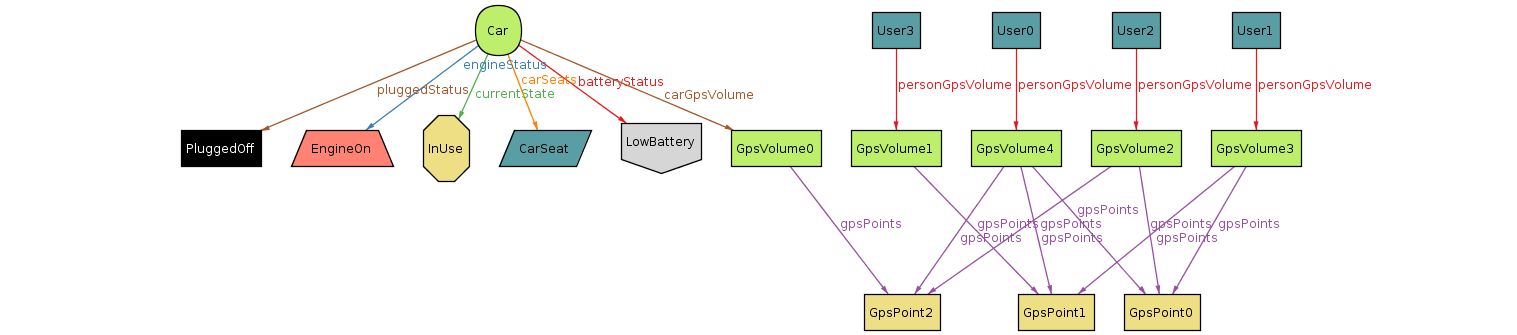
\includegraphics[max size={\textwidth}{\textheight},keepaspectratio]{../Alloy/Exported/Images/Cars_NoPersonInsideInUseCar.png}
\caption{Used cars with no person inside}
\label{fig:CarsNoneInside}
\end{figure}

Another meaningful aspect of our System is the possibility to have perfectly functioning cars whose status is Unavailable. This is surely due to some external Employee who have manually set the status of the Car for whatever reason. This world is shown in Figure \ref{fig:PerfectCarsUnavailable}. 

\begin{figure}[!htbp]
\centering
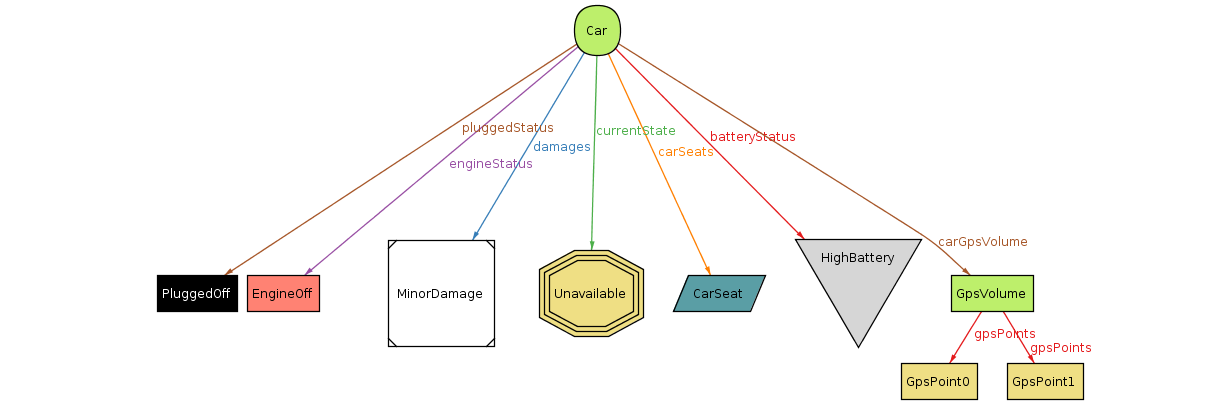
\includegraphics[max size={\textwidth}{\textheight}, keepaspectratio]{../Alloy/Exported/Images/Cars_UnavailableFunctioningCars.png}
\caption{Unavailable functioning cars}
\label{fig:PerfectCarsUnavailable}
\end{figure}

\FloatBarrier
\subsubsection{Areas}
\alloyfile{../Alloy/Exported/Areas.als}

Here we define the CompanyAreas and all the things related to them.

Examples of possible worlds are shown in the following figures. 

In Figure \ref{fig:AreaWorld1} we show a Car which is In Use and at the same time inside a Charging Area without occupying any of its charging slots. This does not come as a surprise: an User can still be inside an Area even if he/she is using the Car. However, we can also notice that, even if the Car is InUse, there is no Person occupying any of the seats. The only User shown in the figure has the same position of the ChargingArea (i.e. he/she is nearby it) and the same position of the Car (i.e. he/she is nearby it).

Figure \ref{fig:AreaWorld2}, instead, shows a Charging Area with a Car inside it. The Car is occupying a ParkingSlot of this ChargingArea. Its status, however, is Unavailable, maybe due to the fact that it has ZeroBattery.

Adding more objects to the model, we can see how things get complicated (but still consistent). Possible worlds are shown in figures \ref{fig:AreaWorld3} and \ref{fig:AreaWorld4}.

Even in this case, we can see in figure \ref{fig:AreasExecutions} how the execution of all checks has not shown any counterexample for our model.

\begin{figure}[!htbp]
\centering
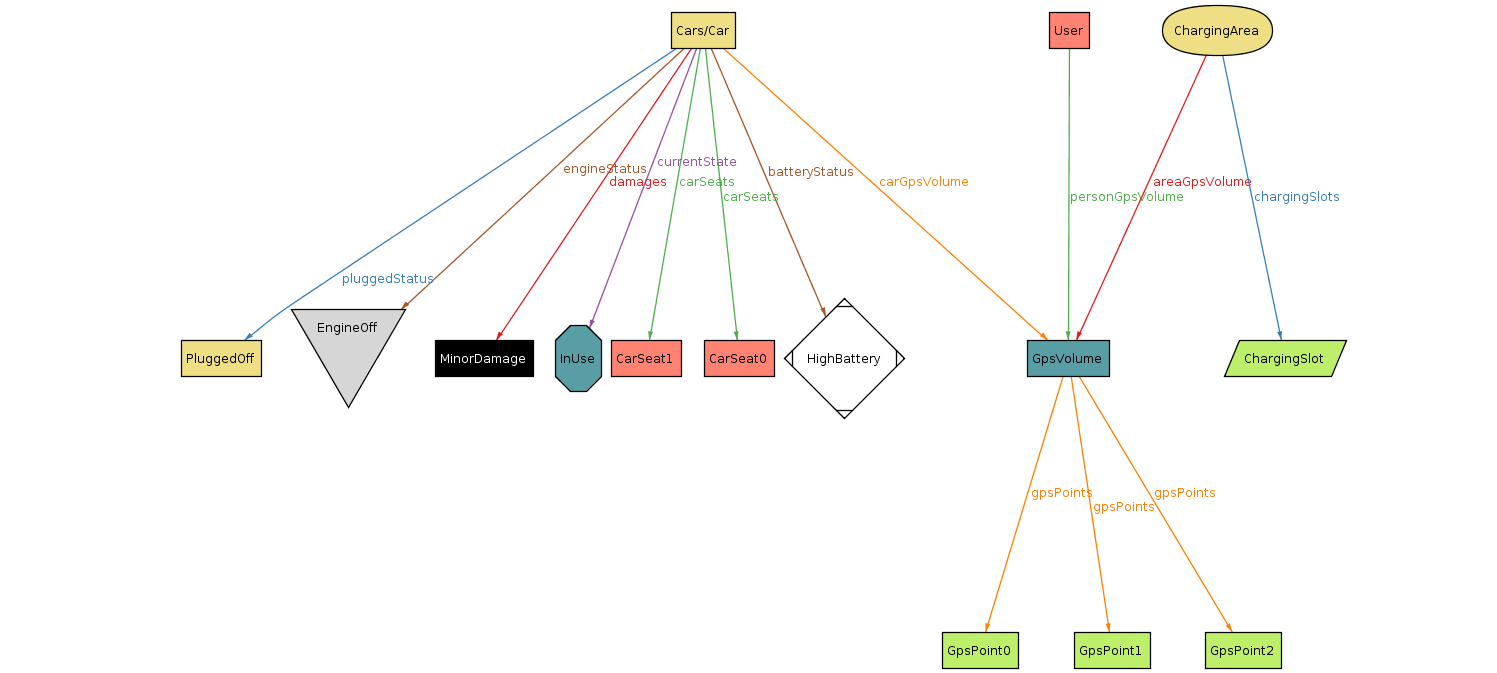
\includegraphics[max size={\textwidth}{\textheight}, keepaspectratio, angle=90, origin=c]{../Alloy/Exported/Images/AreaSimpleWorld.png}
\caption{An Areas World}
\label{fig:AreaWorld1}
\end{figure}

\begin{figure}[!htbp]
\centering
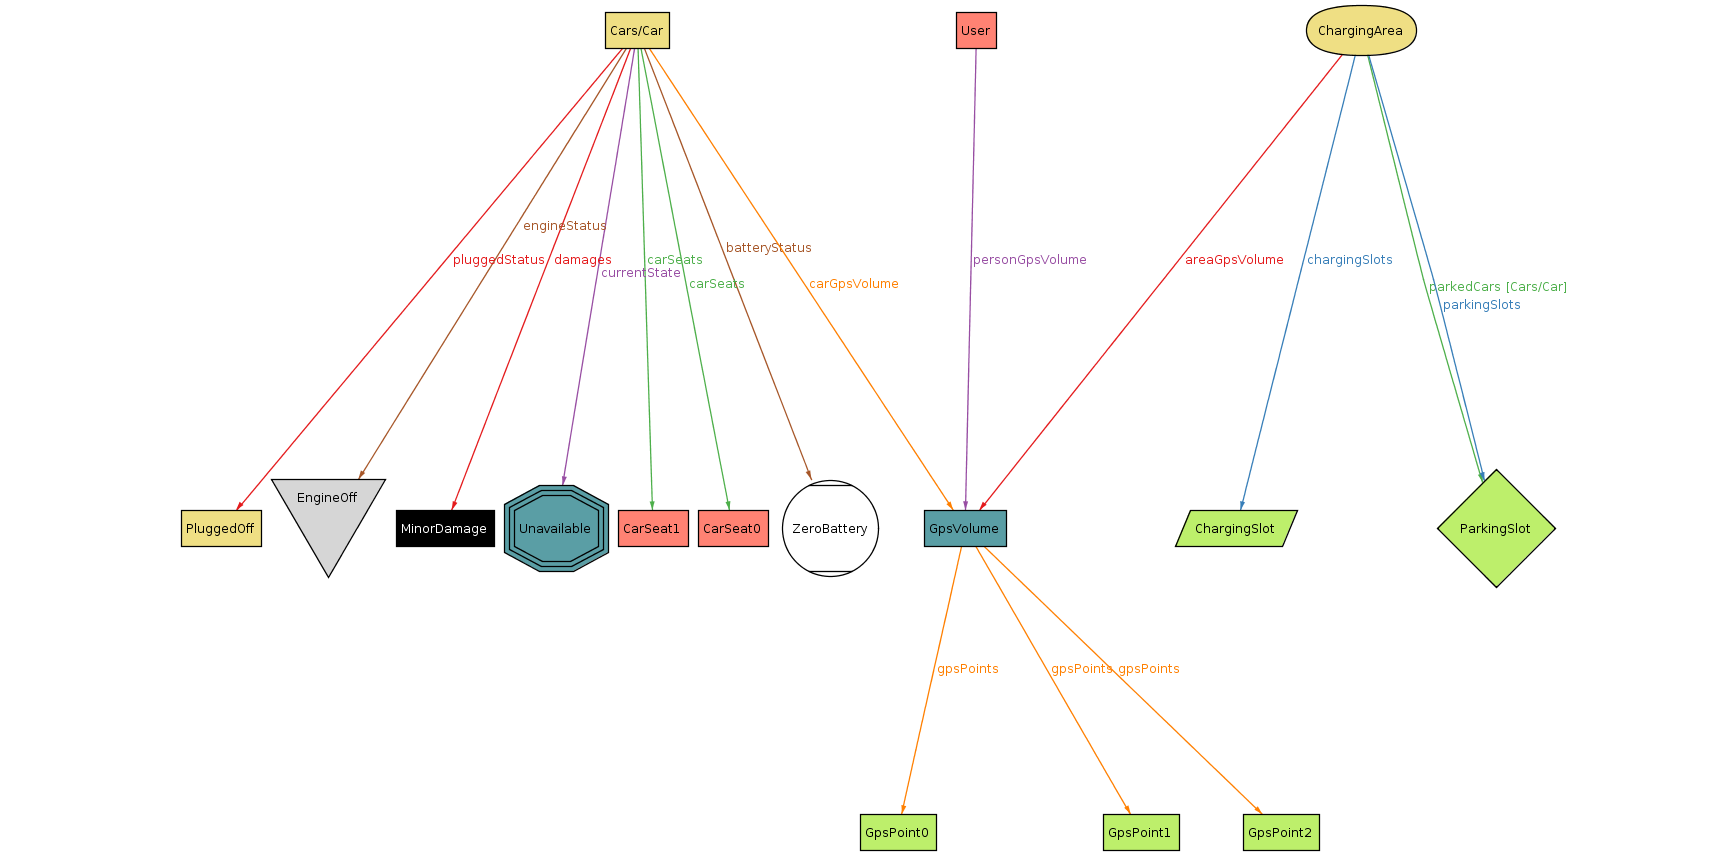
\includegraphics[max size={\textwidth}{0.7\textheight},keepaspectratio, angle=90, origin=c]{../Alloy/Exported/Images/AreaSimpleWorld2.png}
\caption{Another Areas World}
\label{fig:AreaWorld2}
\end{figure}

\begin{figure}[!tp]
\centering
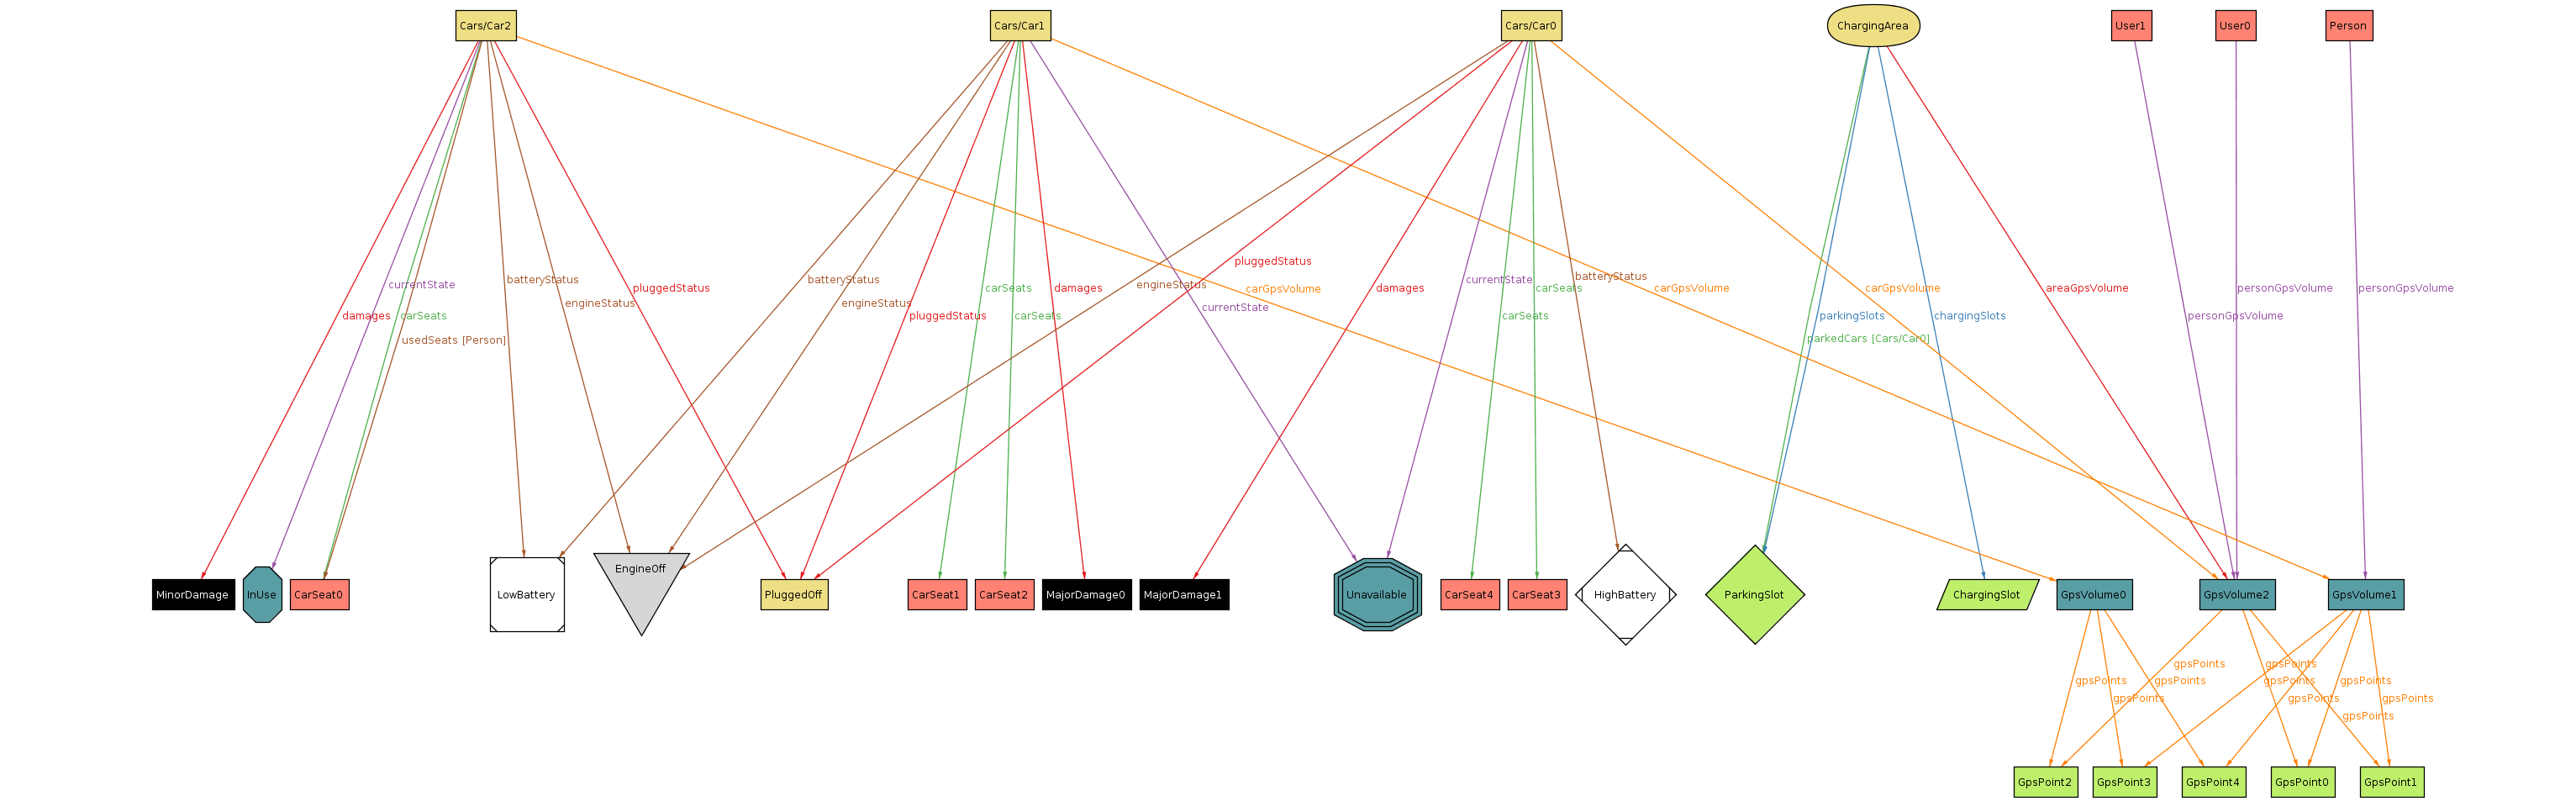
\includegraphics[angle=90, origin=c, max size={\textwidth}{0.7\textheight},keepaspectratio]{../Alloy/Exported/Images/AreaComplexWorld.png}
\caption{A more complicated Areas World}
\label{fig:AreaWorld3}
\end{figure}

\begin{figure}[!tp]
\centering
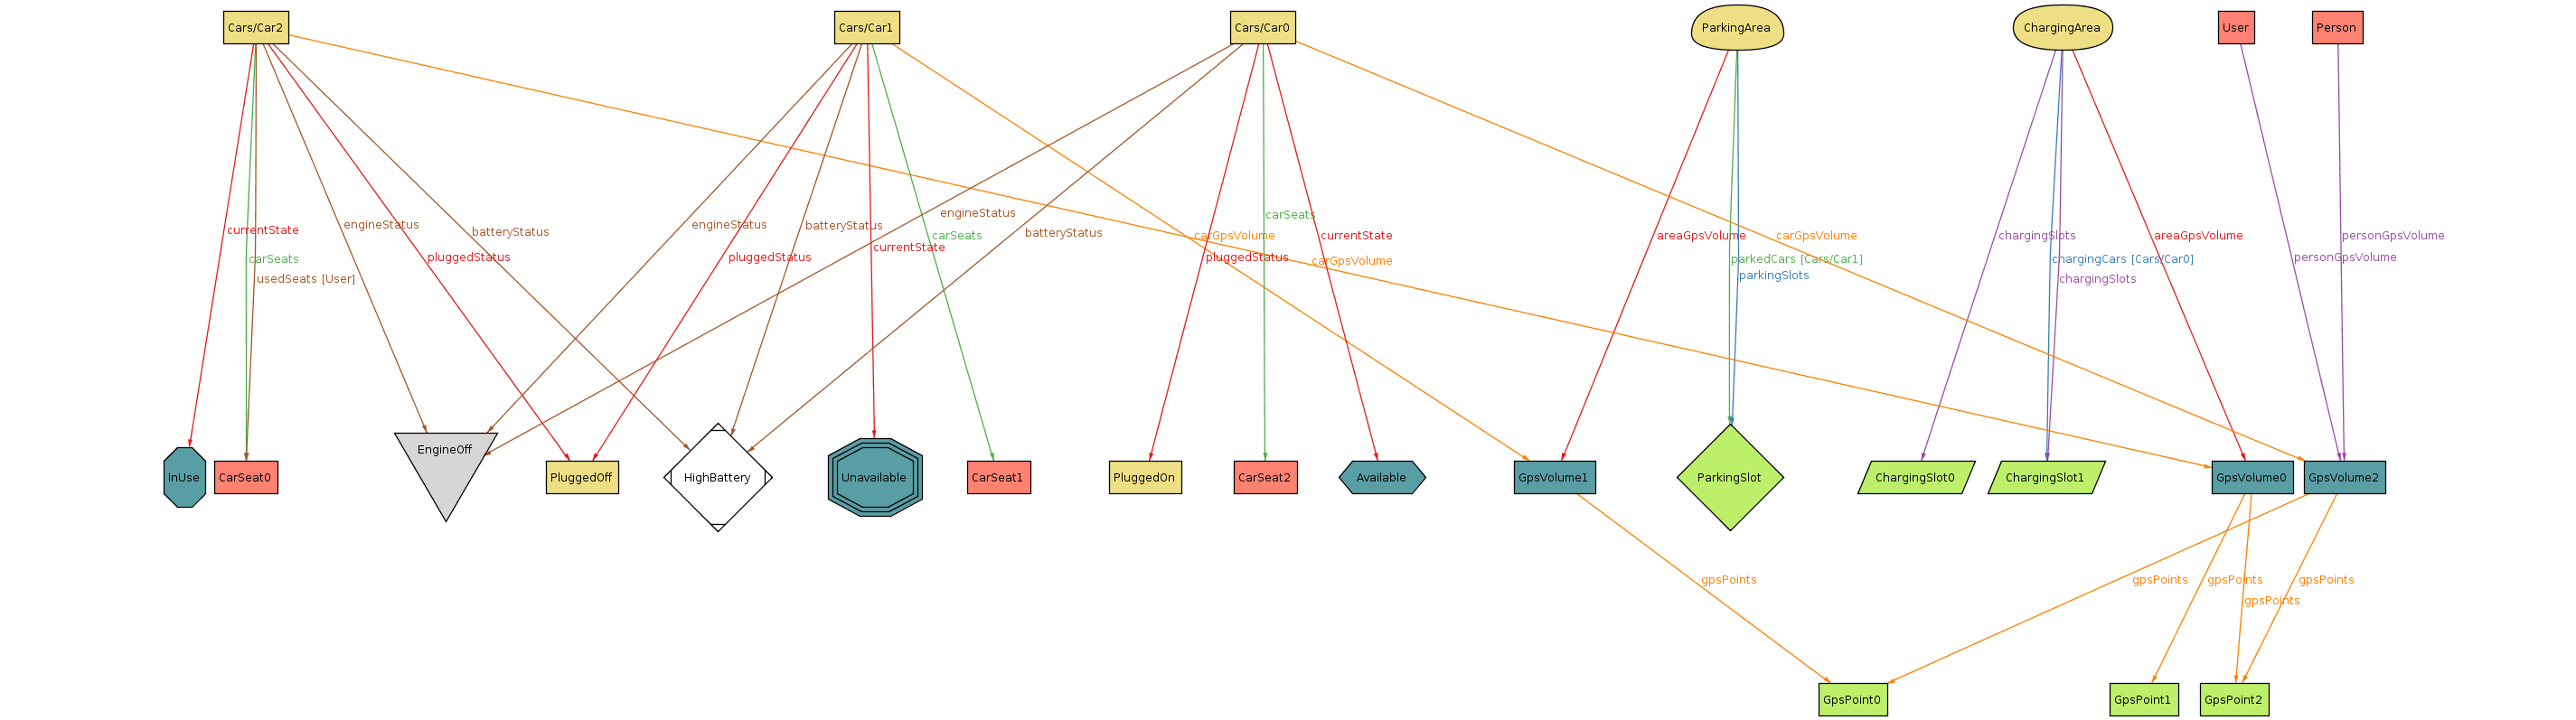
\includegraphics[angle=90, origin=c, max size={\textwidth}{0.7\textheight},keepaspectratio]{../Alloy/Exported/Images/AreaComplexWorld2.png}
\caption{Another more complicated Areas World}
\label{fig:AreaWorld4}
\end{figure}

\begin{figure}[!tp]
\centering
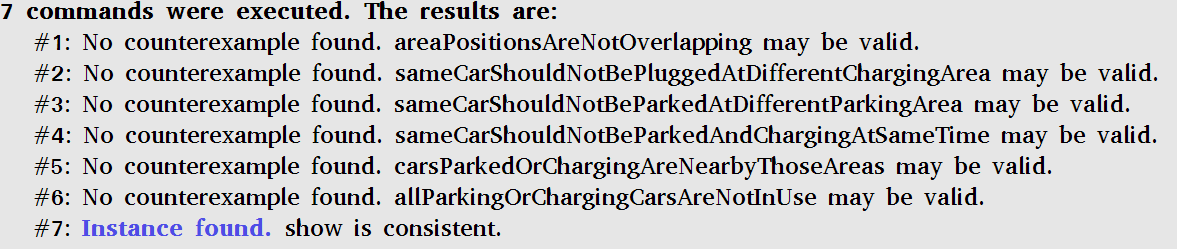
\includegraphics[max size={\textwidth}{0.7\textheight}, keepaspectratio]{../Alloy/Exported/Images/AreasExecutions.png}
\caption{Execution of checks and predicates for areas}
\label{fig:AreasExecutions}
\end{figure}

\FloatBarrier